\section{测度的收敛与极限操作}
\label{sec:measure-convergence}

有了比较两个概率分布的各种指标，自然要问：一整列分布$P_1,P_2,\ldots$什么时候算趋近于某个$P$？
这个问题没有唯一答案，因为“趋近”取决于我们用什么探针去观测。
本节按探针从强到弱排列几种收敛：要求每个事件的误差一致消失的全变差收敛、只要求有界连续观测收敛的弱收敛、再加上距离矩尾部控制的Wasserstein收敛。
然后建立弱收敛下三件常用的事——事件概率怎么读、连续变换是否保持收敛、无界成本的极限下界——并回答“一族分布是否总能挑出收敛子列”。
最后把序列换成随时间变化的测度曲线，提醒不同时间尺度上的极限不能混用。
本节的比较都在同一个固定空间进行；不同空间的对象要先按上一节映到共同空间。

\subsection{测度序列的收敛方式}
\label{sec:measure-sequence-convergence}

\subsubsection{\term{逐集收敛}与全变差收敛}

\paragraph{从比较误差定义趋近}

最强的常用要求是全变差收敛：
\[
 \operatorname{TV}(P_n,P)\to0.
\]
它的含义是：存在一个与事件无关的误差界（就是TV）趋于零，从而\emph{同时}控制所有可测事件。
由前面的不等式，TV收敛等价于Hellinger收敛；KL收敛通过Pinsker界足以推出TV收敛，但反过来不成立（回想$P_\varepsilon=(1-\varepsilon)\delta_0+\varepsilon\delta_1$与$\delta_0$）。

把要求放松一档得到逐集收敛：对每一个\emph{固定}的事件$A$，
\[
 P_n(A)\to P(A).
\]
两者的差别完全在量词上。逐集收敛时，给定精度后需要等多少项$N$可以随事件$A$而变——复杂事件可能要等很久；TV收敛则要求同一个$N$对所有事件一起生效。
因此TV收敛必然推出逐集收敛，反之不然。
不过逐集收敛已经足以控制任意固定的有界可测函数$g$：先用简单函数在$\|g\|_\infty$意义下一致逼近$g$，再利用概率总质量为$1$控制逼近误差，得到
\[
 \int g\,dP_n\to\int g\,dP.
\]

\subsubsection{\term{弱收敛}与连续测试}

\paragraph{弱收敛与位置移动}

再放松一档，连“每个事件”都不要求，只保留对连续观测量的控制。
称$P_n$弱收敛到$P$，记作$P_n\Rightarrow P$，若对每个有界连续函数$\varphi$都有
\[
 \int\varphi\,dP_n\to\int\varphi\,dP.
\]
为什么只用连续函数做探针？因为事件指示函数$\mathbf 1_A$在集合边界上通常是跳变的，分布质量在边界附近的微小挪动会让$P_n(A)$剧烈变化，却不会明显影响任何连续函数的平均。

标准例子正是“质量在位置上不断靠近”。
取
\[
 P_n=\delta_{1/n},\qquad P=\delta_0.
\]
对任意有界连续$\varphi$，积分就是函数值$\varphi(1/n)\to\varphi(0)$，所以$P_n\Rightarrow P$；但事件$\{0\}$的概率始终是$0$而不是$1$，TV距离也始终为$1$。
质量明明在几何上越来越接近，逐事件比较却认为毫无进展——这清楚说明收敛结论依赖于所选标准。

\subsubsection{Wasserstein收敛与矩条件}

\paragraph{弱趋近与距离尾部的共同控制}

弱收敛只管“局部、有界”的观测，不管远处的质量；\term{Wasserstein距离}则会为远距离移动付费。
在Polish空间上，对$P_n,P\in\mathcal P_p(X)$有标准判据
\begin{equation}
 W_p(P_n,P)\to0
 \quad\Longleftrightarrow\quad
 P_n\Rightarrow P
 \ \text{且}\
 \int d(x,x_0)^p\,dP_n\to\int d(x,x_0)^p\,dP.
 \label{eq:measure-wasserstein-criterion}
\end{equation}
——既要在所有有界连续探针上收敛，又要$p$阶矩收敛。
矩条件控制的是“远处的小质量”。
记$z(x)=d(x,x_0)^p$。
先只用弱收敛，把它截断成有界函数$\min(z,R)$，能推出积分在近处（离基点不超过$R$）收敛；真正的差别在截断之外的“尾部”$\int(z-R)_+\,dP_n$。
全矩收敛加上弱收敛，可以推出一个对所有$n$统一成立的尾部估计：先取一个足够大的$R$把\emph{极限测度}的尾部压到很小，再用弱收敛保证$n$足够大时$P_n$在“$R$以外”的概率也很小，两者合起来就把整列的尾部一起压住。
这正是“距离的$p$次方关于这列测度一致可积”的含义；仅有“每个$P_n$自己的矩有限”给不出这种一致性。

\paragraph{小概率远距离的反例}

“每项矩有限”为什么不够？看下面的序列：
\[
 P_n=(1-n^{-p})\delta_0+n^{-p}\delta_n,\qquad P=\delta_0.
\]
远端那一点的概率只有$n^{-p}$，对任意有界连续观测的贡献趋于零，故$P_n\Rightarrow P$；每一项的$p$阶矩也都有限。
但把远端质量搬回原点要走距离$n$，代价是
\[
 W_p(P_n,P)^p=n^{-p}\cdot n^p=1,
\]
永不趋于零。
这把两件事分得很清楚：远端质量的\emph{概率}可以很小，但乘上很大的\emph{距离}后总代价仍是常数；没有对尾部的共同控制，Wasserstein不会收敛。

\begin{figure*}[htbp]
\centering
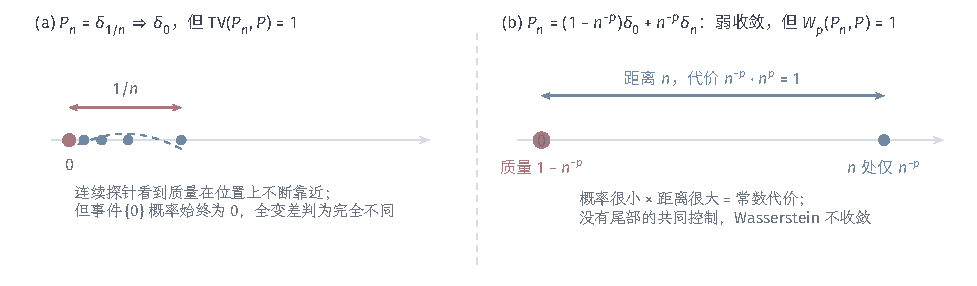
\includegraphics[width=169mm]{figures/01-mathematical-preliminaries-upper/04-space-and-geometry/02-measure-spaces/tikz/convergence-modes/figure.pdf}
\caption{两种“看起来在靠近、却不按更强标准收敛”的典型情形。(a) $P_n=\delta_{1/n}$在几何上不断靠近$\delta_0$，连续探针读数$\varphi(1/n)\to\varphi(0)$，故弱收敛；但事件$\{0\}$的概率始终为$0$，全变差距离恒为$1$。(b) $P_n=(1-n^{-p})\delta_0+n^{-p}\delta_n$弱收敛、每项矩都有限，但把$n$处那一点概率$n^{-p}$搬回原点的$p$次代价$n^{-p}\cdot n^p=1$，故$W_p$不趋于零。}
\label{fig:convergence-modes}
\end{figure*}

\subsection{弱收敛的判据与稳定性}

弱收敛只直接定义在有界连续测试上，实际使用时还想知道：事件概率能不能读、经过映射后还收不收敛、无界成本的极限保不保住下界。
这三者都是弱收敛这同一个概念下的推论，不是新的收敛方式。

\subsubsection{事件概率与边界质量}

弱收敛只在连续函数的积分上成立，可实际问题里我们常想直接读“落在某集合里的概率”。
什么时候这件事合法？答案是：只要极限分布不在该集合的\emph{边界}上放质量。
下面的\term{Portmanteau定理}先给出用开集、闭集表述的形式，事件概率的读法是它的直接推论：
\[
 P_n\Rightarrow P
\]
等价于对所有闭集$C$有$\limsup_nP_n(C)\leq P(C)$，也等价于对所有开集$G$有$\liminf_nP_n(G)\geq P(G)$。
用一句话说就是：当质量整体向$P$靠拢时，落在一个闭集里的概率最终不会超过$P$给它的概率（边界附近的质量可以溜出去），落在一个开集里的概率最终不会少于$P$给它的概率（质量可以从边界溜进来）。
它的实用推论是：如果极限测度不给集合$A$的边界质量，即$P(\partial A)=0$，那么
\[
 P_n(A)\to P(A).
\]

闭集方向可以直观地证明。对闭集$C$，用连续函数
\[
 h_k(x)=\max\{1-k\,d(x,C),0\}
\]
从外面“软包”一层：$h_k$有界连续、在$C$上等于$1$、离开$C$超过$1/k$就降到$0$，且$h_k\downarrow\mathbf 1_C$。
由$\mathbf 1_C\leq h_k$和弱收敛，
\[
 \limsup_nP_n(C)\leq\int h_k\,dP;
\]
再令$k\to\infty$，由支配收敛得到$\limsup_nP_n(C)\leq P(C)$。
开集方向取补集即可。
一般集合用内部$A^\circ$和闭包$\overline A$夹住：
\[
 P(A^\circ)\leq\liminf_nP_n(A)\leq\limsup_nP_n(A)\leq P(\overline A),
\]
只有边界质量为零时两端才相等。
回看$\delta_{1/n}$与事件$\{0\}$：极限测度恰好把质量放在边界$\{0\}$上，条件失败，所以$P_n(\{0\})$不收敛到$P(\{0\})$。
问题的根源始终是探针在集合边界上的跳变。

\subsubsection{连续推前与边缘保持}

弱收敛在连续变换下保持。
设$T:X\to Y$连续且$P_n\Rightarrow P$，对目标端任意有界连续$\varphi$，
\[
 \int\varphi\,d(T_\#P_n)=\int\varphi\circ T\,dP_n\to\int\varphi\circ T\,dP,
\]
因为$\varphi\circ T$仍有界连续。故
\[
 T_\#P_n\Rightarrow T_\#P.
\]
注意结论依赖\emph{连续性}：若$T$只可测不连续，可能失败。例如$P_n=\delta_{1/n}$、$P=\delta_0$，取$T=\mathbf 1_{\{0\}}$，则$T_\#P_n=\delta_0$而$T_\#P=\delta_1$。
连续坐标投影是这一结论的重要应用：若耦合列弱收敛，其两个边缘也分别弱收敛到极限耦合的边缘——这正是后面最优运输计划取极限时仍满足边缘约束的依据。

\subsubsection{\term{下半连续}成本的极限下界}

运输成本通常无界，不能直接当弱收敛的测试，但在下半连续时能保住一个方向的不等式。
所谓\term{下半连续}，直观上就是“极限点处的值不会突然变贵”：当$x_n\to x$时，恒有$c(x)\leq\liminf_n c(x_n)$——成本函数允许在某点向上跳变（如$c(x)=0$只在原点、其余为$1$），但不允许向下塌。
在这个条件下，非负下半连续函数$c$可以用一列有界连续函数从下方逼近：
\[
 c_k(x)=\min\left\{k,\ \inf_y[c(y)+k\,d(x,y)]\right\},
\]
$c_k$的$k$-Lipschitz连续性可直接验证，$c_k\uparrow c$则由下半连续性保证（若某点严格小于$c(x)$，近似取到的点必趋向$x$，与下半连续矛盾）。

设$P_n\Rightarrow P$。先固定$k$用弱收敛，再令$k\to\infty$用单调收敛：
\[
 \int c\,dP=\lim_k\int c_k\,dP
 =\lim_k\lim_n\int c_k\,dP_n
 \leq\liminf_n\int c\,dP_n.
\]
于是
\begin{equation}
 \int c\,dP\leq\liminf_n\int c\,dP_n.
 \label{eq:measure-lsc-portmanteau}
\end{equation}
直觉是：下半连续函数在“极限点处的值不超过附近点的下极限”，积分把这个性质继承下来；极限分布处的最优成本不会比逼近序列的成本下极限更贵。
这里测度本身在变，不能直接套用固定测度的Fatou引理。
这条不等式与紧性配合，正好证明最优运输计划可以取到。

\subsection{\term{一致紧性}与弱子列}
\label{sec:measure-tightness}

前面都是“先有候选极限$P$，再判断$P_n$是否趋近它”。
反过来的问题是：不给定极限，一列概率是否至少能挑出一个收敛子列？
在实轴上有界序列靠紧性总能取子列；一般空间中，类似结论成立的关键是“质量不能跑到任何紧集之外”。

\paragraph{一致紧性与极限子列}

称概率族$\mathcal F$一致紧，若对每个$\varepsilon>0$都能找到\emph{同一个}紧集$K_\varepsilon$，使族中每一个$P$都满足
\[
 P(X\setminus K_\varepsilon)<\varepsilon.
\]
紧集可以随精度$\varepsilon$变，但不能随具体的$P$变——要求的是“一整个族共用一个紧笼子”。
在一般度量空间中“有界”不一定“紧”，所以统一的矩界不能无条件代替一致紧性。

\begin{theorem}[\term{Prokhorov定理}，子列形式]
\label{thm:measure-prokhorov}
在Polish空间上，概率族$\mathcal F$一致紧，当且仅当$\mathcal F$中任意序列都有弱收敛到某个Borel概率的子列。
\end{theorem}

极限概率不必属于原来的族；“某种收敛如何定义”和“是否保证存在收敛子列”是两个独立判断。
质量逃逸的典型反例是$\{\delta_n:n\geq1\}$：每个$\delta_n$本身都是紧支撑的，但不存在一个能同时留住所有$n$的紧集，序列没有弱收敛到概率的子列。

\paragraph{固定边缘下的最优计划}

现在把紧性和下半连续界用到最优运输上，补齐“最优计划存在”的证明三步。
先证明\emph{整个}耦合族$\Pi(P,Q)$一致紧，而不只是某个耦合紧。
给定$\varepsilon>0$，用紧集$K,L$分别把$P,Q$的大部分质量套住：
\[
 P(K^c)<\frac\varepsilon2,\qquad Q(L^c)<\frac\varepsilon2.
\]
对任意$\gamma\in\Pi(P,Q)$，由边缘约束，
\[
 \gamma((K\times L)^c)\leq\gamma(K^c\times Y)+\gamma(X\times L^c)
 =P(K^c)+Q(L^c)<\varepsilon.
\]
于是所有耦合共用同一个紧集$K\times L$。

设成本$c$非负下半连续且至少有一个有限成本耦合，最优值
\[
 I=\inf_{\gamma\in\Pi(P,Q)}\int c\,d\gamma<\infty.
\]
取一列成本趋于$I$的耦合$\gamma_n$；由一致紧性和Prokhorov定理抽出弱收敛子列$\gamma_{n_k}\Rightarrow\gamma$。
连续投影保持边缘，所以$\gamma$仍是$P,Q$的耦合；下半连续积分界给出
\[
 \int c\,d\gamma\leq\liminf_k\int c\,d\gamma_{n_k}=I,
\]
而$\gamma$可行又给出反向不等式，故最小值在$\gamma$处达到。
这就把“紧子列—边缘保持—成本下界”三步接齐。
结论只保证最优\emph{计划}存在，不保证最优\emph{映射}存在；成本也必须下半连续。

\subsection{测度曲线与参数极限}

\paragraph{由序列判据读取时间连续性}

把序号$n$换成连续时间$t$，就得到概率曲线$t\mapsto\mu_t$。
称它弱连续，若每个有界连续探针的读数关于$t$连续，即
\[
 t_n\to t\ \Longrightarrow\ \mu_{t_n}\Rightarrow\mu_t.
\]
若各时刻都在$\mathcal P_p(X)$中，还可要求$W_p(\mu_{t_n},\mu_t)\to0$，由矩判据~\eqref{eq:measure-wasserstein-criterion}，这额外控制了尾部。

点质量曲线$\mu_t=\delta_t$再次显示标准的作用：
\[
 W_p(\mu_s,\mu_t)=|s-t|,
\]
所以它关于$W_p$连续；但$s\neq t$时TV恒为$1$，在全变差意义下处处不连续。
若不同时刻的测度位于不同空间，还要先固定到一个共同空间的表示，才能谈连续性。

\paragraph{固定时刻、有限时域与长时间}

比较一条近似曲线$\mu_t^h$与目标曲线$\mu_t$时，要区分三种越来越强的说法，它们的量词不能互换：
\begin{enumerate}
 \item \emph{固定时刻}：对每个固定$t$，$W_p(\mu_t^h,\mu_t)\to0$；
 \item \emph{有限时域一致}：对每个固定$T$，$\sup_{0\leq t\leq T}W_p(\mu_t^h,\mu_t)\to0$；
 \item \emph{长时间极限}：$t\to\infty$时曲线本身是否趋于某个极限。
\end{enumerate}
取$\mu_t=\delta_0$、$\mu_t^h=\delta_{ht}$（$h>0$）：固定$t$时误差为$ht\to0$，有限区间$[0,T]$上最大误差为$hT\to0$，但在随$h$移动的时刻$t=1/h$误差恒为$1$，所以在$t\geq0$全域上不一致收敛。
这提醒我们：数值近似在每个固定时刻、每个有限时间区间上可靠，并不自动推出长时间结论；演化方程、数值稳定性和极限交换都留给后续问题专门处理。
